% This file was created with matplot2tikz v0.5.3.
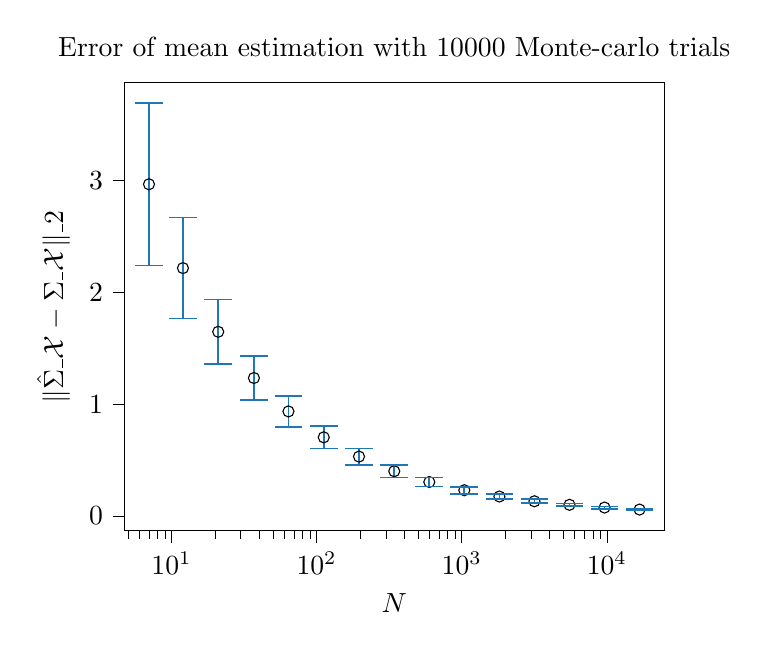
\begin{tikzpicture}

\definecolor{darkgray176}{RGB}{176,176,176}
\definecolor{steelblue31119180}{RGB}{31,119,180}

\begin{axis}[
log basis x={10},
tick align=outside,
tick pos=left,
title={Error of mean estimation with 10000 Monte-carlo trials},
x grid style={darkgray176},
xlabel={\(\displaystyle N\)},
xmin=4.74327639380337, xmax=24803.3195269196,
xmode=log,
xtick style={color=black},
y grid style={darkgray176},
ylabel={\(\displaystyle \|\hat{\boldsymbol{\Sigma}}\_\mathcal{X} - \boldsymbol{\Sigma}\_\mathcal{X}\|\_2\)},
ymin=-0.13262423207483, ymax=3.87655604361312,
ytick style={color=black}
]
\addplot [draw=black, mark=o, only marks]
table{%
x  y
7 2.96644841886547
12 2.21671185618484
21 1.64709208228737
37 1.23397594189885
64 0.935112170973186
112 0.703404726719878
196 0.531310446912574
343 0.400325303184381
598 0.303923396605062
1042 0.230114283599226
1818 0.174038501677559
3170 0.131597391353147
5528 0.0998109498844136
9639 0.0753512175742832
16807 0.0572766951577409
};
\path [draw=steelblue31119180, semithick]
(axis cs:7,2.23857626119455)
--(axis cs:7,3.69432057653639);

\path [draw=steelblue31119180, semithick]
(axis cs:12,1.76497915252549)
--(axis cs:12,2.6684445598442);

\path [draw=steelblue31119180, semithick]
(axis cs:21,1.35747786948254)
--(axis cs:21,1.9367062950922);

\path [draw=steelblue31119180, semithick]
(axis cs:37,1.0374123409997)
--(axis cs:37,1.43053954279801);

\path [draw=steelblue31119180, semithick]
(axis cs:64,0.795915368703914)
--(axis cs:64,1.07430897324246);

\path [draw=steelblue31119180, semithick]
(axis cs:112,0.603021809771917)
--(axis cs:112,0.803787643667839);

\path [draw=steelblue31119180, semithick]
(axis cs:196,0.458345285906057)
--(axis cs:196,0.604275607919091);

\path [draw=steelblue31119180, semithick]
(axis cs:343,0.345034478896582)
--(axis cs:343,0.455616127472181);

\path [draw=steelblue31119180, semithick]
(axis cs:598,0.262460291581848)
--(axis cs:598,0.345386501628276);

\path [draw=steelblue31119180, semithick]
(axis cs:1042,0.198925436760575)
--(axis cs:1042,0.261303130437877);

\path [draw=steelblue31119180, semithick]
(axis cs:1818,0.150584064767169)
--(axis cs:1818,0.197492938587949);

\path [draw=steelblue31119180, semithick]
(axis cs:3170,0.114065796158437)
--(axis cs:3170,0.149128986547856);

\path [draw=steelblue31119180, semithick]
(axis cs:5528,0.0865643002479931)
--(axis cs:5528,0.113057599520834);

\path [draw=steelblue31119180, semithick]
(axis cs:9639,0.0652154542494471)
--(axis cs:9639,0.0854869808991193);

\path [draw=steelblue31119180, semithick]
(axis cs:16807,0.0496112350018946)
--(axis cs:16807,0.0649421553135873);

\addplot [semithick, steelblue31119180, mark=-, mark size=5, mark options={solid}, only marks]
table {%
7 2.23857626119455
12 1.76497915252549
21 1.35747786948254
37 1.0374123409997
64 0.795915368703914
112 0.603021809771917
196 0.458345285906057
343 0.345034478896582
598 0.262460291581848
1042 0.198925436760575
1818 0.150584064767169
3170 0.114065796158437
5528 0.0865643002479931
9639 0.0652154542494471
16807 0.0496112350018946
};
\addplot [semithick, steelblue31119180, mark=-, mark size=5, mark options={solid}, only marks]
table {%
7 3.69432057653639
12 2.6684445598442
21 1.9367062950922
37 1.43053954279801
64 1.07430897324246
112 0.803787643667839
196 0.604275607919091
343 0.455616127472181
598 0.345386501628276
1042 0.261303130437877
1818 0.197492938587949
3170 0.149128986547856
5528 0.113057599520834
9639 0.0854869808991193
16807 0.0649421553135873
};
\end{axis}

\end{tikzpicture}
